%======================================================================
\section{Track ASM --- Assembly}\label{sec:asm}
%======================================================================

FreeCAD 1.1's Assembly workbench already provides joints (Ondsel solver), grounding, exploded views
(\code{Assembly\_CreateView}), a BOM (\code{Assembly\_CreateBom}: Index, Name, File Name, Quantity, plus custom
columns) and kinematic simulation (\code{Assembly\_CreateSimulation}, new in 1.1). This track builds on
those. The file model comes first, because PDM, drawings and BOMs all depend on it.

\begin{epic}{ASM-01}{File model: one part per file}{M1}{\stTodo}{(new)}
SolidWorks-style, as decided: every part is its own \code{.FCStd} with its own P/N, and assemblies
reference parts through \code{App::Link} to external documents with \emph{relative} paths. Tooling:
\textbf{make external} (split the bodies of a multi-body design file into numbered part files and relink),
\textbf{pack and go} (copy an assembly with all its references), and a \textbf{broken-reference resolver}.
\emph{Acceptance:} \code{LE-02001} opens from a moved folder with no broken links.
\end{epic}

\paragraph{Theory: assemblies as a DAG.} Documents form a directed acyclic graph with edges assembly
$\rightarrow$ component and multiplicities $q$. A component \emph{occurrence} is a path
$a_0\to a_1\to\dots\to p$ from the top assembly. Its world placement is the product of the link placements
along the path, $P = P_{a_0a_1}P_{a_1a_2}\cdots P_{a_kp}$. Occurrences, not files, carry joints, colour
overrides and BOM item numbers. Making parts external changes nothing in occurrence space, only which
document owns the geometry. That is why the conversion can be automatic.

\begin{epic}{ASM-02}{Assembly gap audit}{M1}{\stDone}{FCB-P2A-01/02}
Audit current Assembly against a SolidWorks/Fusion checklist and against upstream main. \textbf{Approved
19 Oct 2026 (\S\ref{sec:asm-audit})}; it re-scopes \eref{ASM-03}--\eref{ASM-10}. Three behaviours still need the
screen and are in the test checklist.
\end{epic}

%======================================================================
\subsection{BW-ASM-02 --- Assembly gap audit (approved, 19 Oct 2026)}\label{sec:asm-audit}
%======================================================================

\textbf{Method.} The Assembly workbench in this repository (FreeCAD 1.1.4) was read command by command
(\file{src/Mod/Assembly}), and compared with a SolidWorks/Fusion checklist and with the 97 upstream commits
to \file{src/Mod/Assembly} since the 1.1 release (24 Mar -- 10 Oct 2026, GitHub API). The ``upstream'' column
is what the rebase to main (\eref{FND-03}) brings without any BruceWorx work. Items marked \verify{} need the
GUI and are in the next test session. \textbf{Gate:} the mechanical reviewer approves this list; it then
re-scopes \eref{ASM-03}--\eref{ASM-10}.

\begin{center}
\scriptsize
\setlength{\tabcolsep}{3pt}
\renewcommand{\code}[1]{\texttt{#1}}
\begin{longtable}{@{}>{\raggedright\arraybackslash}p{2.9cm}cc >{\raggedright\arraybackslash}p{4.6cm} >{\raggedright\arraybackslash}p{3.0cm} >{\raggedright\arraybackslash}p{2.3cm}@{}}
\toprule
Capability & SW & Fusion & FreeCAD 1.1.4 (this build) & Upstream main since 1.1 & Gap $\rightarrow$ epic\\
\midrule\endhead
\bottomrule\endfoot
\multicolumn{6}{@{}l}{\textbf{Joints}}\\
Fixed / rigid & \pfull & \pfull & \pfull{} Fixed & --- & ---\\
Revolute, slider, cylindrical, ball & \pfull & \pfull & \pfull{} all four & joint rotate button & ---\\
Planar & \pfull & \pfull & \phalf{} via Distance on two planes (solver \code{ASMTPlanarJoint}) & --- & UX: name it (ASM-03)\\
Tangent / cam & \pfull & \phalf & \phalf{} Distance 0 plane--cylinder = tangent; no cam & --- & cam: later\\
Pin-slot & \pnone & \pfull & \pnone & --- & ASM-03\\
Gear, rack-pinion, screw, belt & \pfull & \phalf & \pfull{} Gears, RackPinion, Screw, Belt & coaxial gear joint; rack-pinion fix & ---\\
Parallel, perpendicular, angle, distance & \pfull & \phalf & \pfull & --- & ---\\
Width / symmetric / path / slot mates & \pfull & \pnone & \pnone & --- & later (not in Fusion)\\
Quick joint (type inferred from picks; SW smart mates) & \pfull & \pfull & \pnone{} one command per type & ``put unconnected part second'' & ASM-03\\
Joint limits & \pfull & \pfull & \phalf{} Length/Angle min--max passed to solver (\code{ASMTTranslationLimit}, \code{ASMTRotationLimit}); honoured while dragging (verified headless); not by a plain solve. Zero from datums: built, section~\ref{sec:joints} & --- & ASM-03\\
As-built joints (no move) & \phalf & \pfull & \pfull{} \emph{Keep parts where they are} (built 19 Oct) & --- & ASM-03\\
Rigid groups & \pfull & \pfull & \pnone & \textbf{RigidGroup (\#29605)} & rebase\\
Edit joint from context menu & \pfull & \pfull & \phalf{} double-click & \textbf{``Edit joint'' entry} & rebase\\
\midrule
\multicolumn{6}{@{}l}{\textbf{Structure}}\\
Insert existing part & \pfull & \pfull & \pfull{} \code{Assembly\_InsertLink} & label fix & ---\\
New part in context & \pfull & \pfull & \pfull{} \code{Assembly\_InsertNewPart} creates \emph{and saves a separate document} --- matches one-file-per-part & joint creation fix & ASM-01 builds on it\\
Sub-assemblies, rigid vs flexible & \pfull & \pfull & \pfull{} \code{AssemblyLink.Rigid} & parent refresh; rigid-change fix & ASM-05 shrinks to verification\\
Grounding & \pfull & \pfull & \pfull & \textbf{grounded parts unmovable} & rebase\\
Component patterns & \pfull & \pfull & \pfull{} BruceWorx link arrays (MOD-01, today) & \textbf{generated arrays + suppressed elements} & align on rebase\\
Mirror components & \pfull & \pfull & \pnone & --- & new, small (ASM-03)\\
Position snapshots / configurations & \pfull & \pfull & \pnone & \textbf{snapshots (\#25384)} & rebase\\
\midrule
\multicolumn{6}{@{}l}{\textbf{Motion and checks}}\\
Free drag with solver & \pfull & \pfull & \pfull{} \code{preDrag}/\code{doDragStep} & island drag (\#30998); transformed-assembly fixes & rebase\\
Kinematic simulation / drive joints & \pfull & \pfull & \pfull{} \code{Assembly\_CreateSimulation} (Angular/Linear motions, formulas) & formula fixes; \textbf{video export (PyAV)} & ROB-05\\
Dynamic motion (gravity, forces, contact) & \pfull & \phalf & \pnone & --- & ASM-10\\
Collision detection during drag (Fusion contact sets) & \pfull & \pfull & \pnone & --- & ASM-06 (+ later)\\
Interference / clearance check & \pfull & \pfull & \pnone{} nothing in \file{src/Mod/Assembly} & --- & ASM-06\\
Degrees of freedom readout & \pfull & \phalf & \phalf & DoF fix with bundled fixed joints & ---\\
\midrule
\multicolumn{6}{@{}l}{\textbf{Documentation output}}\\
Exploded views & \pfull & \pfull & \pfull{} \code{Assembly\_CreateView} & \textbf{move controls (\#30955)} & rebase + ASM-04 presets\\
BOM & \pfull & \pfull & \phalf{} Index, Name, File Name, Quantity automatic; \textbf{custom columns read same-named properties of each part} (\code{BomObject.cpp:283}) & --- & ASM-04 = add P/N, Rev, Material, Mass \emph{properties} to parts (PDM-02)\\
Mass properties of assembly & \pfull & \pfull & \phalf{} \code{MeasureCOM} & --- & MOD-11, ROB-03\\
\midrule
\multicolumn{6}{@{}l}{\textbf{Scale}}\\
Large-assembly / lightweight mode & \pfull & \phalf & \pnone & --- & ASM-08\\
In-context editing & \pfull & \pfull & \phalf{} cross-document \code{SubShapeBinder} & --- & ASM-07\\
Smart fasteners & \pfull & \phalf & \pnone & --- & ASM-09\\
\end{longtable}
\end{center}

\paragraph{What the audit changes.}
\begin{enumerate}
  \item \textbf{Rebase first, then build.} Six rows close by rebasing (rigid groups, snapshots, exploded-view
        controls, edit-joint menu, grounded locking, island drag), and upstream now handles generated arrays and
        suppressed link elements. \eref{FND-03} moves ahead of \eref{ASM-03}.
  \item \textbf{\eref{ASM-04} gets smaller.} The BOM already reads any property by column name, so P/N, Rev and
        Material columns need only the PDM properties on each part (\eref{PDM-02}). Only \emph{Mass} needs new
        code: a computed property kept current on recompute.
  \item \textbf{\eref{ASM-05} becomes verification.} Rigid/flexible sub-assemblies exist
        (\code{AssemblyLink.Rigid}); the epic checks them on \code{LE-02001} and fixes what breaks.
  \item \textbf{\eref{ASM-03} keeps:} quick joint with type inference, pin-slot, mirror components, explicit
        Planar naming, limits verified while dragging, as-built behaviour.
  \item \textbf{Still entirely missing:} interference/clearance (\eref{ASM-06}), dynamic motion
        (\eref{ASM-10}), lightweight mode (\eref{ASM-08}), smart fasteners (\eref{ASM-09}) --- unchanged.
\end{enumerate}

\paragraph{For the next GUI session} (steps 14--16 of section~\ref{sec:tonight}).
\begin{description}[leftmargin=0pt]
  \item[(a) Limits while dragging.] \emph{Dragging} is moving a part with the mouse in the 3D view after it is
        jointed; the solver keeps the joints as you pull. Fusion and SolidWorks stop the part at a joint's limit.
        FreeCAD passes the limits to the solver; whether a drag stops at them is what the step records.
  \item[(b) Joints on pattern instances.] Required (answer, 19 Oct): a joint on a generated bolt must survive
        a change of pattern count while that bolt still exists, and fail with a clear message when it goes.
  \item[(c) Fixed joint placement.] A joint is made by picking a face or edge on each part; the solver then moves
        one part so the two picks line up. ``Stays put'' asks whether a Fixed joint between two parts you have
        already placed keeps them exactly where they are (Fusion calls this an \emph{as-built} joint), or snaps
        the second part so the picks coincide. Both are useful; the step records which FreeCAD does today, and
        \eref{ASM-03} adds the other.
\end{description}

\paragraph{Answered later on 19 Oct.} (a) Drag stays free; limits only when set in the joint, measured from a
datum. (c) Joints keep moving one part to line up the picks; a checkbox keeps parts where they are. Both are built
(section~\ref{sec:joints}); steps 14 and 16 now test them on screen.

\paragraph{Decision (19 Oct).} Audit approved. Part properties must stay open to growth: they now come from a
layered schema instead of code (section~\ref{sec:partprops}).

%======================================================================
\subsection{Part properties that can grow (built 19 Oct 2026)}\label{sec:partprops}
%======================================================================

\textbf{Requirement.} ``Make it so we can expand properties of parts later.'' The properties every part carries
(P/N, revision, description, material, mass, finish, vendor\ldots) are therefore data, not code: a list in
JSON that is read in layers. Adding a property means adding one line to a layer file; FreeCAD, the BOM and the
vault pick it up without a new build.

\begin{center}
\small
\begin{tabularx}{\linewidth}{@{}lX@{}}
\toprule
Layer (read in this order) & Holds\\
\midrule
1. Built in: \file{addons/BruceWorx/config/part\_properties.json} & The nine BruceWorx properties below. Ships with
  the build; not edited by hand.\\
2. Company or vault: e.g.\ \file{<vault>/part\_properties.json} & What your company adds: supplier, lead time,
  RoHS, cost centre\ldots\\
3. User: \file{\textasciitilde/.config/bruceworx/part\_properties.json} & Personal additions while trying something
  out.\\
\bottomrule
\end{tabularx}
\end{center}

\begin{center}
\small
\begin{tabular}{@{}lllll@{}}
\toprule
Property & Type & BOM column & Comes from & Needed at\\
\midrule
\code{PartNumber} & text & \code{.PartNumber} & vault (read-only) & ---\\
\code{Revision} & text & \code{.Revision} & vault (read-only) & ---\\
\code{Description} & text & \code{.Description} & you & submit\\
\code{ItemType} & choice & --- & you (part, assy, COTS, dwg) & ---\\
\code{MaterialName} & text & \code{.MaterialName} & computed: bodies' material & submit\\
\code{Finish} & text & \code{.Finish} & you & ---\\
\code{Mass} & mass & \code{.Mass} & volume $\times$ density & ---\\
\code{Vendor}, \code{VendorPart\-Number} & text & --- & you & ---\\
\bottomrule
\end{tabular}
\end{center}

\paragraph{Rules that keep it safe to grow.}
\begin{itemize}[nosep]
  \item A later layer may \emph{add} properties and may change an existing one's description, default, BOM flag
        or the stage that needs it. It may \emph{not} change a property's type; that would make old files
        unreadable, so the layer is refused with a message naming both files.
  \item Renames are declared (\code{"renamed": \{"Old": "New"\}}); applying the schema moves the value.
  \item Applying never deletes a property it does not know, so a file made with a bigger schema keeps its extra
        values when a smaller one opens it.
  \item A clash with a property FreeCAD already has is reported and left alone. The first real run found one:
        \code{App::Part} already has a \code{Material} link, so ours is \code{MaterialName}.
  \item ``Needed at'' feeds the lifecycle: \code{submit} lists what is still empty before a part can go to review.
\end{itemize}

\paragraph{BOM.} The Assembly BOM prints any property whose column is named \code{.Property}, so the schema
just lists those names. Running it for real exposed an upstream bug: the BOM spreadsheet turned the text
``01'' into the number 1, so revision 01 printed as ``1'' (and a P/N with leading zeros would lose them).
\file{BomObject.cpp} now stores text values as text, the same way it already stores the Index column.

\paragraph{Verified headless.} 12 unit tests (layers, renames, clashes, required stages, enum choices), and a
FreeCAD run on an aluminium plate: mass 135\,g from its 50\,000\,mm$^3$ and Aluminum-6061-T6 density; material
name taken from the body; the BOM row reads \code{LE-01-01001-001 | 01 | Base plate | Aluminum-6061-T6 | Clear
anodise | 135 g}. The Assembly test suite still passes.

\paragraph{Not yet.} A FreeCAD command and panel to apply and edit the properties (today: one line in the Python
console, step 17 of the checklist), and recomputing Mass whenever the body changes (today: whenever the schema is
applied). Both belong to \eref{ASM-04} and \eref{PDM-04}.

%======================================================================
\subsection{Joints: drag, limits from datums, keep parts in place (built 19 Oct 2026)}\label{sec:joints}
%======================================================================

\textbf{Your answers (19 Oct).}
\begin{itemize}[nosep]
  \item Drag must work, with no angle limit unless one is set in the joint.
  \item A limit needs a datum to be measured from.
  \item A new joint moves the parts so the picks line up; a checkbox makes that optional.
\end{itemize}

\paragraph{What FreeCAD 1.1 already did (measured headless).} Limits are off on a new joint. Dragging is free
without them. With limits on, the solver \emph{does} stop a dragged part at them: a 0--90\,$^\circ$ revolute,
dragged to 130\,$^\circ$, stops at 90.000\,$^\circ$. A plain solve does not: a part turned to 120\,$^\circ$ by hand
stays there. What was missing is the reference. FreeCAD measures the angle between the $x$ axes of the two joint
connectors, and the $x$ axis comes from whichever face or edge was picked. So ``0\,$^\circ$'' is wherever the
geometry happens to put it.

\paragraph{Limits from datums.} In the joint panel, \emph{Limits $\rightarrow$ Measured from: Pick datums}, then
pick a planar face, a straight edge, or a datum plane or line on each part. The limits are then measured from the
position where the two datums line up. A door limited to 0--110\,$^\circ$, with the door's face and the wall's face
as datums, reads 0 when it is closed flush. The panel shows the current reading (``Now at 37.0\,$^\circ$''). With no
datums, limits are measured from the joint's own axes, as before. A datum may be given on one side only; the other
side then uses its connector's $x$ axis. \textbf{Which way a datum must face:} for an angle it needs a direction
\emph{across} the axis, so pick a face the axis runs along (the door's face, for its hinge) or an edge square to the
axis. A face square to the axis (the top of the hinge pin) only spins in its own plane and has no angle to read; the
panel and the Report view say so. It does not have to be exactly square: a tilted face is measured by its shadow on
the plane of rotation. For a length limit it is the other way round: faces square to the slide direction.

\begin{figure}[h]
\centering
\begin{tikzpicture}[>=Stealth, scale=1.15]
  \fill[gray!15] (-0.25,-0.25) rectangle (0.25,0.25);
  \draw[thick] (0,0) circle (0.08);
  \node[below left] at (0,0) {\small axis $z_1$};
  % connector 1 x axis
  \draw[->, gray] (0,0) -- (2.6,0) node[right] {\small $x_1$};
  % connector 2 x axis
  \draw[->, gray] (0,0) -- ({2.6*cos(65)},{2.6*sin(65)}) node[above] {\small $x_2$};
  \draw[gray] (0.9,0) arc (0:65:0.9);
  \node[gray] at (1.1,0.5) {\small $\theta$};
  % datum 1
  \draw[->, very thick, bworange] (0,0) -- ({2.2*cos(-25)},{2.2*sin(-25)}) node[right] {\small datum 1, $d_1$};
  \draw[bworange] (0.6,0) arc (0:-25:0.6);
  \node[bworange] at (0.85,-0.17) {\scriptsize $\alpha_1$};
  % datum 2
  \draw[->, very thick, blue!70!black] (0,0) -- ({2.2*cos(105)},{2.2*sin(105)}) node[above left] {\small datum 2, $d_2$};
  \draw[blue!70!black] ({0.5*cos(65)},{0.5*sin(65)}) arc (65:105:0.5);
  \node[blue!70!black] at (-0.02,0.7) {\scriptsize $\alpha_2$};
  % datum angle
  \draw[<->, thick] ({1.6*cos(-25)},{1.6*sin(-25)}) arc (-25:105:1.6);
  \node at (-1.25,1.25) {\small $\theta_d$};
\end{tikzpicture}
\caption{Looking down the joint axis. Each datum sits at a fixed angle $\alpha_i$ in its own connector's frame,
because datum and connector are on the same part. The limit is applied to $\theta_d$, the angle from datum~1 to
datum~2.}
\label{fig:limit-datum}
\end{figure}

\paragraph{The arithmetic.} Turning part~2 by the joint angle $\theta$ turns datum~2 with it, so the datum angle is
\[
  \theta_d = \theta + \alpha_2 - \alpha_1 \qquad\Longrightarrow\qquad \theta = \theta_d + \theta_0,\quad
  \theta_0 = \alpha_1 - \alpha_2 .
\]
Here $\alpha_i$ is the angle of datum $i$'s direction, projected onto connector $i$'s $xy$ plane. The direction is a
face's normal, an edge's direction, or a datum's own $z$. Each $\alpha_i$ depends only on where the datum sits on its
own part, so $\theta_0$ does not change as the parts move. It is stored on the joint as \code{LimitAngleZero}
(read-only). A limit $\theta_d \in [\theta_{\min}, \theta_{\max}]$ becomes $\theta \in [\theta_{\min} + \theta_0,
\theta_{\max} + \theta_0]$ for the solver. Lengths work the same way, with the datums' heights $h_i$ along the axis:
$L_0 = h_1 - h_2$, stored as \code{LimitLengthZero}.

\paragraph{Drag backstop.} The solver stops at limits today, but nothing checked that it does. After each drag step,
BruceWorx now reads every limited joint itself. If a step would take a joint further past a limit, it is cut back:
the move is halved six times from the last good position, so the part stops within $1/64$ of one mouse step of the
limit. A plain solve that leaves a joint outside its limits now prints a warning in the Report view (``Hinge is at
120 deg, outside its limits (0 deg to 90 deg)''). Python can now drive a drag (\code{preDrag}, \code{doDragStep},
\code{postDrag}), which is how all of this is tested without a screen.

\paragraph{Keep parts where they are.} New checkbox in the joint panel, off by default, so a joint still moves one part
to line up the picks. Ticked, the joint is fitted to where the parts are: connector~2's offset takes up the
difference, $O_2' = O_2\,P_2^{-1}P_1$, where $P_i$ are the two connectors' world placements. Nothing moves, and the
joint still works: a revolute made this way turns about connector~1's axis. For a revolute, the angle then reads 0
where the parts were placed, so limits without datums count from the position the parts were built in (Fusion's
\emph{as-built} joint). The setting is stored on the joint (\code{KeepPosition}); ticking or unticking it while the
panel is open redoes the joint from the parts' original places. It is shown for Fixed, Revolute, Cylindrical, Slider
and Ball joints.

\paragraph{Verified headless.} 7 new Assembly tests (\file{AssemblyTests/TestBWJoints.py}), all passing with the 8
existing ones:
\begin{itemize}[nosep]
  \item a free drag to 170\,$^\circ$ and $-120\,^\circ$ without limits;
  \item a 0--90\,$^\circ$ limit stops a drag at 90 and at 0;
  \item the reading equals the face-to-face angle worked out from the geometry, at five angles;
  \item a 0--30\,$^\circ$ limit from two face datums stops a drag at 30 and at 0 measured face to face;
  \item no datums gives zero offsets;
  \item a joint moves the part by default, and with \emph{Keep parts where they are} it does not move it, even after a
        solve, and still turns about the joint.
\end{itemize}
The panel itself (checkbox, \emph{Pick datums}, reading) needs the screen: steps 14 and 16 of
section~\ref{sec:tonight}.

\paragraph{Still in \eref{ASM-03}.} Quick joint with type inference, pin-slot, limit sliders in the 3D view, datums on
the assembly origin or a third part (today both datums are on the joint's own two parts), and continuous angles past
$\pm 180\,^\circ$ (today a limit range lies within one turn).


\begin{epic}{ASM-03}{Joint UX \& limits}{M1}{\stProg}{FCB-P2A-03/04}
A pick-two-features \textbf{quick joint} that infers the joint type (cylinder + cylinder $\rightarrow$
revolute, plane + plane $\rightarrow$ planar, and so on), keyboard shortcuts, and \textbf{limit sliders} that the
solver honours while dragging. \textbf{Built 19 Oct (\S\ref{sec:joints}):} limits measured from datums, a drag
backstop at the limits, and \emph{Keep parts where they are}.
\emph{Acceptance:} the 2-DOF arm is assembled with quick joints, and limits stop the drag.
\end{epic}

\begin{epic}{ASM-04}{Exploded views \& BOM}{M1}{\stProg}{FCB-P2A-05/06}
Exploded-view presets, and a BOM with \textbf{P/N, Rev, Description, Material, Mass, Qty}, in
\emph{indented}, \emph{top-level} and \emph{flattened (parts only)} forms, exported to CSV. Configurations are
resolved per component (\eref{MOD-03}). The same BOM feeds the drawing table (\eref{DRW-02}) and Ops
(\eref{PDM-06}).
\textbf{Started 19 Oct 2026:} the columns come from the part-property schema (\S\ref{sec:partprops}), with
Mass and Material computed.
\emph{Acceptance:} the \code{LE-02001} BOM matches a hand count; the flattened BOM sums quantities.
\end{epic}

\paragraph{Theory: BOM explosion.} With edge multiplicities $q_{uv}$ in the assembly DAG, the total quantity
of part $p$ under top assembly $t$ is the sum over all paths of the product of multiplicities,
\[
  Q_t(p) = \sum_{\pi:\,t\rightsquigarrow p}\ \prod_{(u,v)\in\pi} q_{uv},
\]
computed in $O(|V|+|E|)$ by dynamic programming in topological order, $Q(v)=\sum_{u\to v}Q(u)\,q_{uv}$ with
$Q(t)=1$. The \emph{indented} BOM lists paths, and the \emph{flattened} BOM lists $Q_t(p)$ for leaf parts.
\emph{Where-used} (\eref{PDM-06}) is the same traversal on the reversed graph.

\begin{epic}{ASM-05}{Sub-assemblies}{M1}{\stTodo}{FCB-P2A-07}
Rigid vs.\ flexible sub-assemblies. A flexible one exposes its internal joints to the parent's solver; a
rigid one moves as one body. A fix-up macro converts between them.
\emph{Acceptance:} a flexible sub-assembly articulates inside \code{LE-02001}; a rigid one does not.
\end{epic}

\begin{epic}{ASM-06}{Interference \& clearance}{M1}{\stTodo}{FCB-P2A-08}
List every \textbf{clash} (positive common volume), \textbf{contact} (touching faces, zero volume) and
\textbf{clearance violation} (minimum distance below a threshold) between occurrences. Results are
highlighted in the view, with an ignore list for intended press fits and threads. The ECAD enclosure fit
(\eref{ECD-04}) reuses it.
\emph{Acceptance:} the bolt example in Figure~\ref{fig:clash} reports one clash, 4.0\,mm deep and 78.5\,mm$^3$.
\end{epic}

\begin{figure}[ht]
\centering
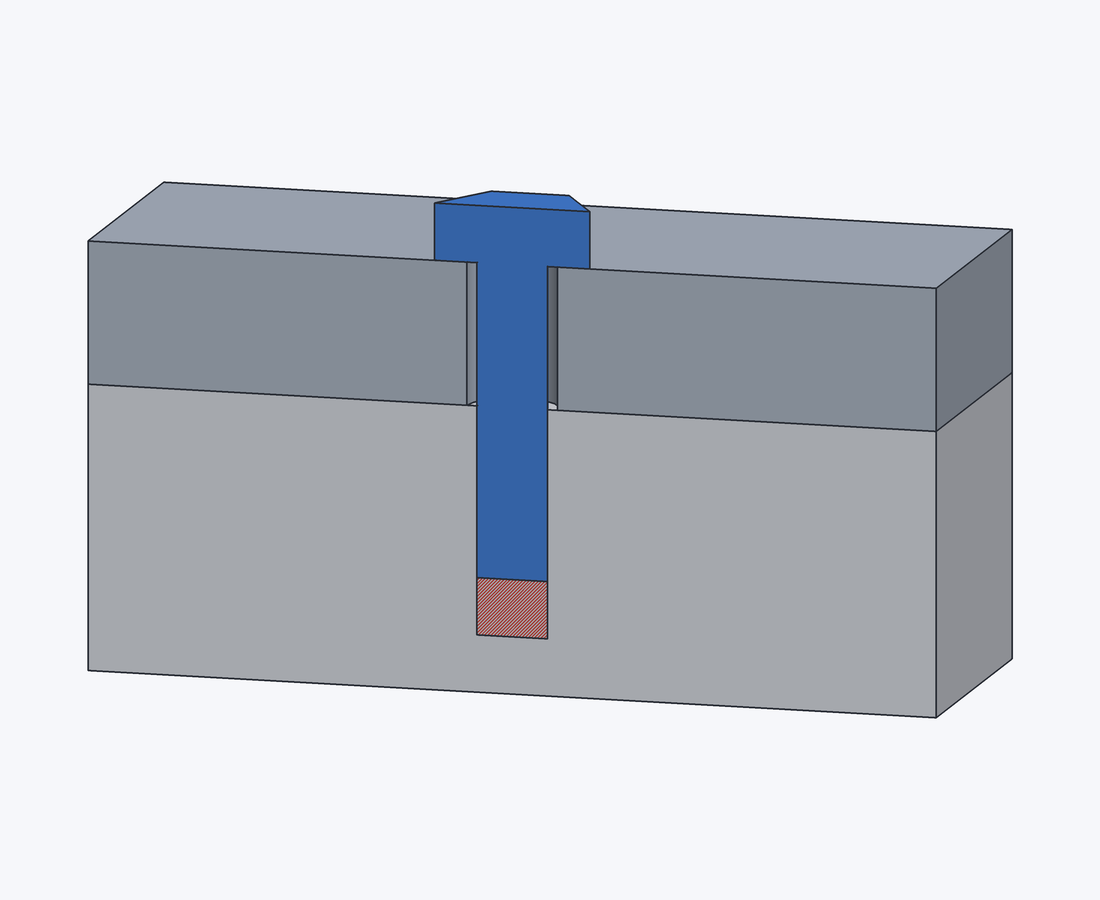
\includegraphics[width=0.5\linewidth]{fig/interference.png}
\caption{Half section of an M5 bolt that is 4\,mm too long for its 12\,mm blind hole. The clash volume
(red) is the Boolean common of bolt and block: 78.54\,mm$^3$ $=\pi\cdot2.5^2\cdot4$, computed in headless
FreeCAD. The section itself is the kind of view \eref{MOD-11} keeps in the model.}
\label{fig:clash}
\end{figure}

\paragraph{Theory: broad and narrow phase.} Checking all $\binom n2$ pairs exactly is too slow for a robot with
hundreds of parts. A \emph{broad phase} sorts the axis-aligned bounding boxes on each axis and sweeps,
reporting only pairs whose intervals overlap on all three axes. That takes $O(n\log n+k)$ for $k$ candidate pairs.
The \emph{narrow phase} runs the exact Boolean common (clash volume) or \code{distToShape} (clearance)
only on candidates. Contacts are separated from clashes by a volume tolerance $\varepsilon_V$ and a
distance tolerance $\varepsilon_d$. Pairs on the ignore list (threads, press fits) are filtered by occurrence
path, so they stay ignored after the assembly is rebuilt.

\begin{epic}{ASM-07}{In-context editing}{M5}{\stTodo}{(new)}
Edit a part while it is shown inside the assembly, referencing other parts' geometry (Fusion's in-place edit,
SolidWorks' in-context features). References become cross-document \code{SubShapeBinder}s and update when
the referenced part changes. They can be \textbf{locked} (frozen) or \textbf{broken}. A dashboard lists all
external references.
\emph{Acceptance:} bracket holes follow a moved motor mount across files.
\end{epic}

\begin{epic}{ASM-08}{Large-assembly mode}{M5}{\stTodo}{(new)}
Open a full robot quickly. That means \textbf{lightweight} loading (display data without the feature tree),
\textbf{selective open} (choose the sub-assemblies to load), cached tessellation, and level of detail
for small parts. The spike measures FreeCAD's existing partial-document loading for links first \verify.
\emph{Acceptance:} an assembly of more than 500 parts opens within a target set by the spike.
\end{epic}

\begin{epic}{ASM-09}{Smart fastener mating}{M5}{\stTodo}{FCB-P2R-04}
Select a hole pattern and a fastener type. The command recognises the holes (\eref{MOD-04} recognition,
\eref{MOD-05} data), picks size and length, inserts linked fasteners (and washers and nuts), and joints them.
This matches SolidWorks Toolbox smart fasteners and its 2026 fastener recognition.
\emph{Acceptance:} bolting a motor mount places and joints all its screws in one command.
\end{epic}

\paragraph{Theory: length selection.} For a through-bolt with clamp (grip) thickness $g$ into a tapped or
insert hole of usable depth $h$, the required engagement is $e\ge k\,d$, with $k\approx1.5$ in aluminium
and plastics, or the insert length for heat-set inserts. The chosen standard length is the smallest catalogue
length $L$ with
\[
  g + e \;\le\; L \;\le\; g + h - c ,
\]
where $c$ is the bottom clearance. If the set is empty, the command reports the conflict instead of
choosing. Figure~\ref{fig:clash} shows the failure it prevents.

\begin{epic}{ASM-10}{Dynamic motion study}{M5}{\stTodo}{FCB-P2A-10}
Beyond kinematic animation: \textbf{gravity, applied forces and torques, motor profiles, springs and
dampers, and contact}, integrated over time, with plots (position, velocity, reaction forces, motor
torque) and video export. The spike checks how much of the Ondsel (MbD) solver's dynamics can be used
\verify.
\emph{Acceptance:} the arm swinging under gravity matches the analytic pendulum period within 2\,\%.
\end{epic}

\paragraph{Theory: constrained multibody dynamics.} With generalised coordinates $\mathbf q$, mass
matrix $M(\mathbf q)$, applied forces $\mathbf Q$ and joint constraints $\Phi(\mathbf q,t)=\mathbf 0$,
\[
  M\ddot{\mathbf q}+\Phi_{\mathbf q}^{\!\top}\boldsymbol\lambda=\mathbf Q,\qquad \Phi(\mathbf q,t)=\mathbf 0,
\]
an index-3 differential-algebraic system. The Lagrange multipliers $\boldsymbol\lambda$ are the joint reaction
forces, which is what users want plotted to size motors. It is solved by index reduction to
$\Phi_{\mathbf q}\ddot{\mathbf q}=-(\Phi_{\mathbf q}\dot{\mathbf q})_{\mathbf q}\dot{\mathbf q}-2\Phi_{\mathbf qt}\dot{\mathbf q}-\Phi_{tt}$
with Baumgarte stabilisation, or with a generalised-$\alpha$ integrator on the index-3 form. Validation uses a
pendulum, $T=2\pi\sqrt{I_O/(m g\ell)}$.
